% Apparent sequence-model contribution depends strongly on negative-set construction
% Preprint / journal submission. Subject area Bioinformatics. Licence CC BY 4.0.
%
% Build:  pdflatex paper && pdflatex paper      (no bibtex; references are a thebibliography)
% Figures are expected in ./figures/ as PDF. See manuscript/build.sh, which copies them from
% results/figures/ so that this directory is a self-contained submission package.
\documentclass[11pt]{article}

\usepackage[utf8]{inputenc}
\usepackage[T1]{fontenc}
\usepackage{lmodern}
\usepackage[margin=1in]{geometry}
\usepackage{graphicx}
\usepackage{booktabs}
\usepackage{amsmath}
% amssymb for \mathbb, used by the estimand definitions in Methods.
\usepackage{amssymb}
\usepackage[numbers,sort&compress]{natbib}
\usepackage[colorlinks=true,allcolors=blue]{hyperref}
% PDF metadata are written explicitly so that indexing does not depend on the typeset title.
\hypersetup{
  pdftitle={Apparent sequence-model contribution depends strongly on negative-set
            construction: a calibration across 94 ENCODE eCLIP datasets},
  pdfauthor={Nirmalkumar Thirupallikrishnan Kesavan (ORCID 0009-0002-9977-1739)},
  pdfsubject={Calibration of negative-set construction in RNA-binding-protein sequence model
              benchmarks},
  pdfkeywords={RNA-binding proteins; eCLIP; negative sets; benchmark calibration; sequence
               models; ENCODE},
  pdfcreator={pdfLaTeX}
}
% lineno redefines footnotes, so apply only the compatible microtype patches.
\usepackage[patch={item,eqnum,verbatim}]{microtype}
% Allow long repository URLs to break without requiring an additional package.
\def\UrlBreaks{\do\/\do\-\do\.\do\_\do\a\do\b\do\c\do\d\do\e\do\f\do\g\do\h\do\i\do\j\do\k\do\l\do\m\do\n\do\o\do\p\do\q\do\r\do\s\do\t\do\u\do\v\do\w\do\x\do\y\do\z}
\Urlmuskip=0mu plus 1mu\relax
% Preprint conventions. Line numbers and 1.5 spacing are what reviewers ask for on a
% manuscript under consideration; both are cosmetic and can be dropped for a camera-ready
% version by commenting out these three lines.
\usepackage[modulo]{lineno}
\usepackage{setspace}
\onehalfspacing

% \doi is used in the text (Data availability) as well as the bibliography, so it has to be
% defined in the preamble rather than alongside thebibliography, which is \input last.
\providecommand{\doi}[1]{\href{https://doi.org/#1}{doi:#1}}

% Starred sections get no hyperref anchor and no PDF bookmark, so a link into the back matter
% lands on whatever page precedes it and the document outline stops at the Conclusion. This adds
% both. The .toc it writes is otherwise unused, there being no \tableofcontents, but hyperref
% builds the bookmark tree from it.
\newcommand{\backsection}[1]{%
  \phantomsection\addcontentsline{toc}{section}{#1}\section*{#1}}

% Tighter float placement: this paper is table-heavy and LaTeX will otherwise push everything
% to the end.
\renewcommand{\topfraction}{0.9}
\renewcommand{\textfraction}{0.08}
\renewcommand{\floatpagefraction}{0.8}

% A handful of long unbreakable tokens (model slugs, command lines) sit in otherwise fine
% paragraphs. Widen the tolerance slightly rather than rewording around typesetting.
\tolerance=1500
\emergencystretch=2em

% The title states the result that transfers across estimators and external validation.
\title{\bfseries Apparent sequence-model contribution depends strongly on negative-set
construction: a calibration across 94 ENCODE eCLIP datasets}

\author{Nirmalkumar Thirupallikrishnan Kesavan\\[2pt]
\normalsize Department of Mechanical and Industrial Engineering, College of Engineering\\
\normalsize Northeastern University, Boston, MA, USA\\
\normalsize \texttt{thirupallikrishnan.n@northeastern.edu}\\[1pt]
\normalsize ORCID: \href{https://orcid.org/0009-0002-9977-1739}{0009-0002-9977-1739}}

\date{}

\begin{document}
\linenumbers
\maketitle

% The abstract is intentionally concise; detailed sensitivity analyses remain in Results.
\begin{abstract}
\noindent
Sequence models for RNA-binding proteins (RBPs) are evaluated against constructed negative
windows, but the influence of negative selection on estimated model contribution is poorly
characterised. I compared GC-matched, dinucleotide-matched and bias-aware negatives across 94
ENCODE eCLIP datasets, using the same source peaks and holding the model class,
chromosome-blocked folds and estimator fixed. Contribution was defined as incremental AUROC over a
19-feature composition baseline.

For a 4-mer model, contribution varied 4.84-fold across protocols (95\% CI 3.98--5.81) with the
primary cross-fitted estimator and 5.42-fold (4.43--6.58) with the conventional two-stage
estimator. Two-stage spans ranged from 3.7- to 7.4-fold across the 4-mer, a convolutional neural
network and SpliceBERT. Replacing GC-matched with dinucleotide-matched negatives reduced the
4-mer AUROC from 0.798 to 0.688 in all 94 datasets, while increasing its contribution from
0.027 to 0.066 in 88 datasets.

The conventional estimator also produced a positive null contribution of $+0.011$ to $+0.014$
for a 2-mer model whose features were contained in the baseline. Cross-fitting the score
covariate reduced this floor by at least 95\% in every protocol. In 135 held-out datasets from
an independently constructed benchmark, the two negative sets produced a 1.66-fold
cross-fitted span (95\% CI 1.40--1.98), or 1.67-fold (1.40--2.00) after chromosome-blocked
refolding. Protocol dependence replicated, whereas the inverse relation between apparent
difficulty and contribution did not.

Incremental performance therefore depends on both the negative-set protocol and the baseline
used to define it. I recommend cross-fitting score covariates, reporting composition-only
performance under the same protocol, and avoiding direct comparisons of contributions
estimated under different negative-set constructions.
\end{abstract}

\noindent\textbf{Keywords:} RNA-binding proteins; eCLIP; benchmarking; negative-set
construction; sequence composition; incremental value; AUROC

\section{Introduction}
Sequence models of RNA-binding protein (RBP) occupancy are commonly evaluated by the area under
the receiver operating characteristic curve (AUROC) on held-out sequence windows. Positive
windows are defined by crosslinking assays such as eCLIP
\citep{vannostrand2016,vannostrand2020}; negative windows must instead be constructed. Typical
choices include unbound regions from the same transcripts \citep{maticzka2014},
composition-matched genomic windows \citep{khan2021}, and sites bound by other RBPs
\citep{horlacher2023}. This choice determines the discrimination problem presented to the
model, but it is often described only briefly.

The consequences can be substantial. \citet{horlacher2023} evaluated eleven RBP-prediction
methods across hundreds of CLIP-seq experiments and showed that apparent performance depended
on the negative-set definition. They proposed a bias-aware protocol in which sites bound by
other RBPs serve as negatives, thereby reducing some of the compositional and accessibility
differences between bound sites and genomic background. Related sensitivity has been observed
in transcription-factor binding prediction: models trained with dinucleotide-shuffled
negatives transferred less effectively to held-out high-quality data than models trained with
genomic negatives \citep{tourne2026}. More generally, evaluation-set construction can inflate
apparent accuracy, alter method rankings and change the interpretation of genomic prediction
models \citep{grimm2015,whalen2022,krutzfeldt2020,cohendavidi2024}.

Raw AUROC combines two quantities: the signal captured by a model and the difficulty of the
classification task defined by the benchmark. Uniform genomic negatives, for example, may
differ markedly from crosslinked positives in nucleotide composition. A classifier can then
achieve a high AUROC by exploiting composition alone. GC matching reduces one component of
this difference, but GC content constrains only one linear combination of the sixteen
dinucleotide frequencies. The remaining compositional degrees of freedom may still support
substantial discrimination. Similar dependence of incremental performance on baseline strength
has been described outside genomics \citep{pencina2012}.

I therefore distinguish a model's \emph{apparent AUROC} from its contribution beyond an
explicit composition baseline. Apparent AUROC is the performance reported under a particular
negative-set protocol. The nested contribution is the difference between two pooled
out-of-fold AUROCs: one from a logistic model containing composition features and the sequence
model's score, and one from the same composition features alone. Both models are fitted on the
same observations and folds. The primary baseline contains mono- and dinucleotide frequencies
and sequence entropy, represented by 19 columns after removing redundant frequency levels.
Because the resulting contribution depends on the baseline used to define it, I also evaluate
higher-order composition models.

This analysis uses 94 ENCODE eCLIP datasets and three negative-set protocols: GC-matched
genomic windows, dinucleotide-matched genomic windows, and a bias-aware set drawn from sites of
other RBPs assayed in the same cell line. The protocols differ not only in composition matching
but also in transcript-region constraints and transcriptional status. Across protocols I use
the same source peaks and hold the model class and hyperparameters, chromosome-blocked fold
assignment and estimator implementation fixed; the sequence model and composition baseline are refitted within each
protocol. I examine a 4-mer logistic regression, a 7089-parameter convolutional neural network
and a fully fine-tuned 19.78~M-parameter SpliceBERT model \citep{chen2024}.

Within the study panel, stricter composition matching lowered apparent AUROC while increasing the
estimated contribution beyond composition. The magnitude of this contribution varied several-
fold across protocols and was comparable to the variation produced by changing model class.
The dependence persisted across alternative performance measures and baseline orders, although
its magnitude changed. I further identified a positive null floor in the conventional
two-stage estimator and showed that cross-fitting the score covariate largely removed it.
Finally, an analysis of 135 held-out datasets from \citet{horlacher2023} reproduced the
protocol dependence but not the inverse relation between apparent difficulty and contribution.

Together, these results motivate three reporting practices: evaluate the composition baseline
under the same protocol as the sequence model, cross-fit score covariates when estimating
incremental performance, and avoid comparing contributions obtained under different
negative-set constructions. The aim is not to identify a universally preferred negative set,
but to make the scientific question posed by each benchmark explicit and its measurements
interpretable.


\section{Materials and Methods}
\subsection{Panel selection}

Candidate experiments were every released ENCODE eCLIP experiment in K562 and HepG2 (139 and 105
respectively). Where a protein had several peak files we took the one with the most biological
replicates, breaking ties by ENCODE's \texttt{preferred\_default} flag, and required
\texttt{output\_type=peaks}, \texttt{assembly=GRCh38}, \texttt{status=released} and
\texttt{file\_format=bed}. Every candidate was preprocessed under both composition-matching
protocols; datasets retaining at least 400 out-of-fold scored pairs were eligible.

The study panel was then defined once by the dinucleotide arm, which is the stricter control:
the 189 eligible datasets were sorted by pair count with a stable sort and every second one
retained, giving 95 datasets over 79 proteins. The set was halved rather than taken whole
because the sweep trains three model classes over five folds and three protocols, and the full
eligible set did not fit the compute budget the retained panel already consumes. Given that a
reduction was necessary, we sampled systematically by rank instead of taking the largest $N$,
because AUROC correlates with dataset size in these data, negligibly for
the composition baseline (Pearson $r$ on $\log_{10} n$ of $-0.04$ in the GC arm) but strongly
for the models, reaching $0.70$ for SpliceBERT under dinucleotide matching, so a size-truncated
panel would confound panel membership with the measured quantity; the retained panel spans the
0th to 99th percentile of the candidate size distribution. Of the 95, 94 also cleared the floor
in the GC arm and constitute the paired panel used for every three-protocol result, giving 282
protocol-dataset cells. All 95 are used only for the comparison of standalone model AUROCs
quoted in the Introduction, which needs no GC-arm counterpart. Panel membership was written once
to a manifest that every downstream stage reads. Supplementary Table S1 lists every dataset with
its ENCFF file and ENCSR experiment accession.

Sixteen proteins are assayed in both cell lines and contribute two datasets each, fifteen of
them in the paired panel. All headline intervals therefore resample proteins rather than
datasets.

\subsection{Windows}

Positive windows are 101~nt centred on the midpoint of each peak interval. Peak width and the
significance columns are unused: we applied no further $p$-value, $q$-value or fold-change
filter, because ENCODE's released \texttt{peaks} files are already thresholded and across our 95
files the minimum log2 fold-enrichment is 3.0000 and the minimum $-\log_{10}p$ is 3.0003, which
are the criteria of \citet{vannostrand2020}; 91.7\% of the 463{,}091 peaks carry ENCODE's IDR
label. The positive set is therefore every peak ENCODE called and no weaker ones. Minus-strand
windows are reverse-complemented
and transcribed to RNA, so every sequence is the strand the protein sees. Windows containing an
ambiguous base, falling outside the assembly, duplicating an existing window by start
coordinate, or carrying no region annotation are dropped and counted. Analysis is restricted to
chr1 to chr22 and chrX; chrY and all scaffolds and alternates are excluded.

Region class is assigned from GENCODE v45 \citep{frankish2023} as the first of (5$'$UTR,
3$'$UTR, CDS, non-coding exon, intron) whose interval set contains the window midpoint. Region
intervals were built from all transcripts with no
gene-type filter and merged, with strand disregarded at this step; introns were computed as the
gaps between consecutive exons.
GTF 1-based inclusive coordinates are converted to 0-based half-open.

\subsection{The three negative-set protocols}

Each protocol produces one negative per positive. All three use a single random stream seeded at
7 per protein.

\paragraph{GC-matched.} Candidates are windows of the same region class on the same chromosome,
at least 500~nt from any peak of the target protein, drawn with probability proportional to the
length of each free interval. A candidate is accepted if its GC content is within 0.05 of the
positive's. The matcher relaxes: after 25 unsuccessful draws the tolerance doubles to 0.10, and
if 40 draws fail the best candidate seen is accepted provided it is within three times the
nominal tolerance, that is 0.15. Only the target protein's own
peaks are excluded, so a GC-matched or dinucleotide-matched negative may be another protein's
binding site. The negative inherits the positive's strand label; the consequences are quantified
in the Results.

\paragraph{Dinucleotide-matched.} Positives are grouped by region and chromosome, and for each
group a candidate pool of $\max(1500,\, 8n)$ windows is sampled from the same free intervals the
GC matcher draws on: same region class, same chromosome, and at least 500~nt from any peak of the
target protein, the exclusion applied through the same code path and the same configured distance.
The two composition-matched protocols therefore share one candidate universe and differ only in
the statistic they match on. For each positive the nearest
unused candidate is assigned greedily under the $L_1$ distance over the sixteen dinucleotide
\emph{counts}, searched with a $k$-d tree over the forty nearest neighbours. The distance is over counts, not frequencies, because integer
distances are exactly representable, and each candidate carries an additional
tiebreak column that increases strictly with genomic position and is
bounded below 0.5, so it can never reorder candidates whose integer distances differ but resolves
exact ties by position. Without both devices the choice among tied candidates depends on the
floating-point behaviour of the $k$-d tree implementation and a different negative is selected
for about 8\% of pairs between CPU architectures. Assignment is greedy, not optimal;
achieved distances are reported so the quality of the approximation is visible. Used coordinates
are tracked across all groups, because one interval can be annotated as both a non-coding exon
and a 3$'$UTR and so appear in two region pools. No maximum distance is imposed.

\paragraph{Bias-aware (other RBPs' sites).} Following \citet{horlacher2023}, negatives for a
target are the positive windows of the other panel proteins assayed in the same cell line,
sampled 1:1 without replacement, excluding any donor window within 500~nt of any of the target's
own positive windows. Our version deviates from \citet{horlacher2023} in two ways: our donor
pool is the study panel (40 to 48 donor proteins per dataset, median 45) and not a full
ENCODE survey, and exclusion is by distance from the target's 101~nt windows, not from its
full peak intervals. Both the donor pool and the target's positives are read from the GC arm's
window tables, so this arm inherits the GC matcher's retained positive set and its pair count is
identical to that arm's. Sampling is performed within fold, so every pair stays inside one
cross-validation fold. These negatives are transcribed, accessible to crosslinking and
strand-correct by construction, and are not composition-matched in any respect.

\paragraph{What each protocol holds fixed.} The three protocols are not three settings of one
knob, and the difference changes how their results should be read. Both composition-matched
protocols draw candidates of the same transcript region class as the positive, so the region
label carries no information about the class. The bias-aware protocol matches fold only, which
leaves region free; how far region separates the two classes there is measured in
Section~\ref{sec:region}. Only the bias-aware
protocol's negatives are transcribed RNA, and conversely 67.6\% of GC-arm negatives lie in loci
not transcribed on the strand the window is labelled with. Section~\ref{sec:region} bounds what
the region asymmetry contributes; the strand and
transcription controls in the Results bound the other two; these are the tables the
repository names \texttt{strand\_placebo} and \texttt{transcription\_placebo}.

\subsection{Achieved match quality}

Achieved matching was quantified over every pair in each arm, 456{,}734 in the GC and
bias-aware arms and 457{,}998 in the dinucleotide arm (Table~\ref{tab:match}).

\begin{table}[htbp]
\centering
\caption{Achieved match quality between each positive and its assigned negative, all pairs.
Columns two to five describe the absolute GC difference between the pair; $L_1$ is over the
sixteen dinucleotide frequencies, on a 0 to 2 scale.}
\label{tab:match}
\begin{tabular}{lcccccc}
\toprule
arm & med.\ $|\Delta$GC$|$ & p90 & p99 & max & within 0.05 & med.\ $L_1$ \\
\midrule
GC-matched & 0.0297 & 0.0495 & 0.1089 & 0.1486 & 94.8\% & 0.500 \\
dinucleotide-matched & 0.0198 & 0.0693 & 0.1485 & 0.4159 & 85.0\% & 0.220 \\
bias-aware & 0.1387 & 0.3169 & 0.4555 & 0.6733 & 20.4\% & 0.700 \\
\bottomrule
\end{tabular}
\end{table}

The GC matcher holds its nominal tolerance for 94.8\% of pairs and its observed maximum,
0.1486, sits at the 0.15 fallback cap. ``Dinucleotide-matched'' likewise means a median $L_1$
of 0.220 rather than zero: the matcher improves composition distance 2.27-fold relative to the
GC arm but does not eliminate it. The bias-aware arm is not composition-matched at all, with a
median GC gap 4.7 times the GC arm's.

\subsection{Cross-validation}

Evaluation is grouped 5-fold cross-validation over whole chromosomes. The chromosome-to-fold map
is frozen once for all datasets in both cell lines, so the fifteen proteins measured in both
lines are evaluated on the same chromosomes and a between-line difference cannot be a partition
artefact. The map was chosen by random-restart hill climbing on peak counts only, never on labels
or model output, minimising the summed squared deviation from equal mass per fold with every
dataset weighted equally; it was required to beat round-robin assignment, to hold the median
per-dataset maximum deviation at or below 0.05, and to place no more than half of any dataset's
data in one fold. Fold $i$ is the test fold, fold $i+1 \bmod 5$ is validation and the remaining
three train, so each fold is test once, validation once and training three times, and no
additional data is spent on model selection.

Every window is scored exactly once out of fold and all AUROCs are computed on the pooled
out-of-fold score vector. Pooling, instead of averaging per-fold AUROCs, makes the
estimate invariant to fold size; the least balanced dataset places 0.42 of its data in a single
fold.

Leakage between folds was audited by exact 32-mer sharing, not by clustered sequence
identity. A 101~nt window contains 70 distinct 32-mers, and two unrelated sequences share one
with negligible probability, so a shared 32-mer indicates common origin. Over all 94 datasets,
holding fold 0 out, a median of 2.0\% of held-out windows shared any 32-mer with a training
window (maximum 24.3\%), a median of 0.08\% shared more than half of their 32-mers, and the
median dataset contained no window sharing more than 90\%. Chromosome grouping therefore leaves
a small residue of homologous sequence across folds, which is the quantity a sequence-identity
clustering step would remove.

\subsection{The composition baseline and the nested contribution}

The composition baseline is a 19-column design matrix: three mononucleotide frequencies, fifteen
dinucleotide frequencies and the Shannon entropy of the window's base composition. One level is
dropped from each frequency family because frequencies sum to one and retaining all of them
makes the design singular; dropping a level does not change the space the block spans. Every
column is standardised over the whole dataset, not within fold; the transform is
label-free and identical in both terms of every comparison, so it cannot manufacture a
contribution. GC content is not a feature: it is the spanned combination C$+$G, and
mononucleotide counts are almost, but not exactly, marginals of dinucleotide counts: over a
window of length $L$ the dinucleotide counts sum to $L-1$ and recover each base's count only up
to whether the terminal base is that base. The linear block therefore has rank 18 and not 15,
with a median 0.14\% of each mononucleotide column's variance lying outside the span of the
dinucleotide columns (maximum 0.25\% over 25 datasets), and the entropy column adds a
nineteenth, nonlinear direction. What the two protocols constrain is nonetheless asymmetric by
construction, and that asymmetry is what the design argument rests on: GC matching fixes a
single linear functional of local composition, whereas dinucleotide matching fixes all fifteen
degrees of freedom of the dinucleotide simplex, so it leaves the baseline strictly less
compositional variation to exploit. The baseline is refit on each protocol's own windows and is
never carried between protocols.

The nested contribution of a model is
\begin{equation*}
\mathrm{AUROC}(\text{composition} + \text{standardised model score}) -
\mathrm{AUROC}(\text{composition alone}).
\end{equation*}
Both terms were fitted by $L_2$-penalised logistic regression ($C=1$, lbfgs, at most 3000
iterations), once per fold on that fold's training rows, and evaluated as pooled out-of-fold
linear predictors on identical rows and folds. The model-score column is the out-of-fold score
for every row, training rows included, so the nested model is never fitted on an in-sample
score; had it been, the fitted and evaluated covariate would sit on different scales and the
mismatch would grow with how much the underlying model overfits, which differs sharply between
a 256-column penalised logistic and a fully fine-tuned transformer. The two were compared by DeLong's paired
estimator \citep{delong1988}, in the $O(n\log n)$ midrank form of \citet{sun2014}. The paired
estimator is necessary here because the two score vectors are fitted on overlapping training
data and evaluated on identical rows, so they are strongly correlated and treating them as
independent would overstate the variance of their difference: the median DeLong standard error
of the difference is 0.26 times what independence gives. Confidence intervals on a single
dataset's contribution are Wald intervals on the DeLong standard error.

\citet{demler2012} show that DeLong's test is not valid for strictly nested models, because
under the null the added predictor's contribution degenerates. Two things bound the exposure
here. The panel-level intervals, which carry every headline, do not use the DeLong standard
error at all; they are protein-clustered bootstrap intervals over per-dataset point estimates.
And where the DeLong standard error is used, for the per-dataset significance counts, it is
conservative relative to the recommended alternative: a penalised likelihood-ratio test on the
same fits calls 89 of 94 datasets significant in the GC arm against DeLong's 80. A third
feature of the design might have cut the other way and does not: negatives are matched 1:1 to
positives, so the rows are paired, while DeLong treats the two classes as independent samples.
Resampling matched pairs instead reproduces the DeLong standard error to within 1\% (median
ratio 0.99 over 30 datasets), so the matching needs no correction.

Both arms are evaluated out of fold. An in-sample composition AUROC compared against an
out-of-fold model AUROC flatters composition sufficiently to reverse the comparison on
individual datasets.

\subsection{Models}

\paragraph{4-mer logistic regression.} Raw 4-mer counts over the RNA sequence (98 per window,
256 columns) into $L_2$-penalised logistic regression ($C=1$). One model per fold, out-of-fold
score taken as the linear predictor. The $k$-mer order is 4, and the contrast is
positive at every order from 3 to 6.

\paragraph{Convolutional network.} A DeepBind-style architecture \citep{alipanahi2015}:
convolution (4 to 16 channels, width 12), ReLU, max-pool 4, convolution (16 to 32, width 8),
ReLU, global max-pool over position, dense 32 to 64, ReLU, dropout 0.5, dense 64 to 1. 7089
parameters, all trained from scratch. Global max-pooling makes the model
position-invariant, which is necessary here because exploratory analysis placed the
discriminative signal approximately 15~nt off centre, varying by protein.

\paragraph{SpliceBERT.} The pretrained nucleotide language model of \citet{chen2024},
\texttt{multimolecule/\allowbreak splicebert}, fully fine-tuned; 19.78~M parameters, all trainable. The
classification head is a mean pool over real nucleotide tokens, masking classification,
separator and padding tokens, then dense to 128, ReLU, dropout 0.3, dense to 1. Weights are
baked into the container image at build time.

Both neural models: AdamW, weight decay 0.01, batch size 32, binary cross-entropy, single
precision, at most 12 epochs with early stopping on validation AUROC at patience 4, best
checkpoint restored before test scoring. Learning rate $10^{-3}$ for the head and
$3\times10^{-5}$ for a fine-tuned encoder. Nominal epochs overstate the training
performed: the median best epoch for SpliceBERT was 3 and most runs stopped by epoch 6 or 7,
whereas the convolutional network typically ran the full 12. Initial weights were drawn before
the seed was set, so initialisation is unseeded across all 2830 committed fold-runs, that is two
models by five folds by 94 datasets in the GC and bias-aware arms and 95 in the dinucleotide
arm; the measured
cost is a per-dataset standard deviation of 0.006 to 0.010 in the nested contribution, inducing
about 0.001 on a 94-dataset mean against a reported interval half-width of about 0.008. The
convolutional and transformer arms were trained on different accelerators, which changes
floating-point summation order and is covered by the same measurement.

\subsection{Inference}

Because fifteen of the 79 proteins contribute two datasets each and the within-protein
correlation of the primary contrast is 0.92, every headline interval is a percentile interval
from a bootstrap that resamples \emph{proteins} and takes all datasets of each sampled protein,
4000 draws. Dataset-level intervals are 1.05 to 1.23 times narrower and are not reported as
headline values.

Two analyses are confirmatory and are the only ones we adjust. The first is the primary
contrast, the difference in nested contribution between protocols, which the study was built to
estimate. The second is the recommendation test of Section~\ref{sec:recommendation}, whose two
falsifying criteria were fixed before the external data were scored and whose interval is
Bonferroni-corrected over the three protocol pairs. Everything else here is exploratory. That
includes the baseline attribution, the family partition, the order-three contrast, the
within-panel reversal and the caliper-matched nulls, all of which we report as point estimates
with intervals rather than as decisions, and none of which is adjusted for the number of
analyses performed. Readers should treat an exploratory interval that just excludes zero
accordingly.

Per-dataset significance counts are also reported at a design effect of 1.35 applied to the
DeLong standard error, which is intended to cover two things the estimator does not: that it
conditions on two score vectors as fixed when both are fitted, and that it treats spatially
clustered windows as independent. We measured both components instead of assuming them
(\texttt{scripts/design\_effect.py}). Resampling whole genomic blocks inflates the standard
error of the contribution by a median factor of 1.100, and the factor is insensitive to block
length, moving only to 1.104 at 100~kb and 1.138 at 1~Mb, so the objection that a 10~kb block
is smaller than a gene does not bite. Permuting the model score within fold and refitting gives
1.048. The measured product is therefore 1.15 rather than 1.35. We retain 1.35, because it is
the more conservative of the two and because the count it produces was fixed before the
components were measured; a reader who prefers the measured figure should read 75 of 94 rather
than 72 of 94 below. This is one of two quantities in the paper that the verification harness
cannot check
from the released evidence, because the block bootstrap needs the genomic coordinates that the
published per-window score files do not carry.

\subsection{Reproducibility}

All published values are reproduced offline by a single command against committed evidence. The
harness runs 706 numeric assertions against a frozen expectations file, and the harness asserts
that no
fewer than that number ran, so a check cannot silently skip. Two assertions are
stronger than regression gates: 285 published AUROCs are rebuilt from committed per-example
scores to a maximum absolute difference of $2.2\times10^{-16}$, and the headline contrast is
rebuilt from raw sequence to $1.2\times10^{-6}$. Per-window out-of-fold scores for all three
model classes are committed, so every cell of the model-class comparison is recomputable from the
repository alone, and is not asserted against a hand-entered table.

Three devices guard against platform-dependent results: dinucleotide distances are computed on
integer counts, candidate ties are broken by genomic position, and the panel sort is stable.
Each was added after an observed discrepancy between CPU architectures or between runs.

Analyses used NumPy \citep{numpy}, SciPy \citep{scipy}, scikit-learn \citep{sklearn}, PyTorch
\citep{pytorch} and Matplotlib \citep{matplotlib}.


\section{Results}
\subsection{Apparent difficulty and measured contribution move in opposite directions}

Holding the model, the positives, the folds and the estimator fixed and changing only how the
negative windows were built gives three different pictures of the same 4-mer on the same 94
datasets (Table~\ref{tab:three}, Figure~\ref{fig:three}).

\begin{table}[htbp]
\centering
\caption{The same model on the same positives under three negative-set protocols, $n=94$
datasets. Only the construction of the negative windows differs.}
\label{tab:three}
\begin{tabular}{lccc}
\toprule
protocol & composition alone & apparent AUROC & nested contribution \\
\midrule
dinucleotide-matched & 0.6274 & 0.6937 & $+0.0663$ \\
GC-matched & 0.7827 & 0.8092 & $+0.0265$ \\
bias-aware (other RBPs' sites) & 0.8248 & 0.8370 & $+0.0122$ \\
\bottomrule
\end{tabular}
\end{table}

Moving from GC-matched to dinucleotide-matched negatives lowers apparent AUROC by 0.1095, and it
does so in 94 of 94 datasets (paired Wilcoxon $p<10^{-15}$). The same change raises the measured
contribution from $+0.0265$ to $+0.0663$, a contrast of $+0.0398$ $[+0.0325, +0.0477]$
(protein-clustered, positive in 88 of 94). A reader comparing the two benchmarks by headline
AUROC would conclude the model had got worse. A reader comparing what the model added would
conclude it had got nearly three times better. Both readings are correct about their own
quantity, and they point in opposite directions.

The bias-aware protocol is where this becomes a problem for practice. Drawing negatives from
other proteins' binding sites is designed to remove the compositional and accessibility
artefacts that genomic-background negatives carry, and it does: those negatives are transcribed,
crosslink-accessible and strand-correct by construction, and no composition matcher touches
them. We pre-registered the prediction that composition would fall toward 0.5 under this
protocol, because both classes are real crosslink sites, and that the measured contribution
would rise. Both halves were wrong. Composition alone is the \emph{highest} of the three arms at
0.8248, the discrimination is the \emph{easiest} of the three by apparent AUROC at 0.8370, and
the measured contribution is the \emph{lowest} at $+0.0122$, 0.53 times the GC arm (geometric
mean over the 83 datasets positive in both arms; the ratio of panel means is 0.46). The reason is
visible in hindsight and is itself a result: different RBPs bind compositionally different sites,
so telling one protein's sites from another's is largely a composition task.

The ordering is therefore monotone in measured difficulty and not in how principled the protocol
sounds. Ranked by composition alone, by apparent AUROC or by contribution, all three orderings
agree. ``Harder negatives reveal more of what a model adds'' is exactly true. What is false is
the inference that a bias-aware protocol is harder: it is the easiest of the three, and it
reveals the least.

Two further features of Table~\ref{tab:three} matter for interpretation. Composition alone beats
the 4-mer outright in 29 of 94 datasets under GC matching. And the 4-mer's contribution is
significantly positive in 80 of 94 datasets, falling to 72 of 94 at the design effect measured
for these data (Methods), so on roughly a quarter of the panel the model adds nothing detectable
over composition under the protocol in common use.

The \emph{sign} of the GC-versus-dinucleotide contrast is implied by the design, and we state
this here rather than in a limitations paragraph. The composition baseline occupies the fifteen
degrees of freedom of the dinucleotide simplex; GC matching constrains one linear functional of
that space and dinucleotide matching constrains all fifteen, so the arm that controls more of
the baseline must leave the baseline weaker and the model more room. Only the \emph{magnitude}
is informative. What the design does not imply is the bias-aware arm's position: that protocol
constrains \emph{none} of the fifteen degrees of freedom, its negatives are not
composition-matched in any respect (median absolute GC gap 0.1387 against the GC arm's 0.0297),
and it nonetheless has the highest composition baseline of the three. No degrees-of-freedom
argument predicts that, and it is what breaks a purely circular reading of the table.

\paragraph{Artefact controls.} Two alternative explanations were pre-registered and bounded
against matched placebos, each with twenty placebo seeds. A strand-annotation artefact, arising
because a matched negative inherits its positive's strand label, accounts for $-0.0055$
$[-0.0089, -0.0022]$ of the contrast, leaving 85.4\% standing. Negatives drawn from
untranscribed loci account for $-0.0043$ $[-0.0069, -0.0018]$, leaving 89.7\%; 40.1\% of
negatives lie in untranscribed loci, but that fraction is balanced across the two arms to within
$1.2\times10^{-5}$ ($p=0.64$), and a confound present equally in both arms cannot manufacture a
difference between them. One argument needs no placebo: GC-matched negatives are 42.8\% sense
against 47.4\% in the dinucleotide arm, higher in 37 of 40 datasets ($p=5.0\times10^{-9}$), so
the spurious directional cue is stronger in the arm with the \emph{smaller} contribution and
works against the reported direction.

\begin{figure}[htbp]
\centering
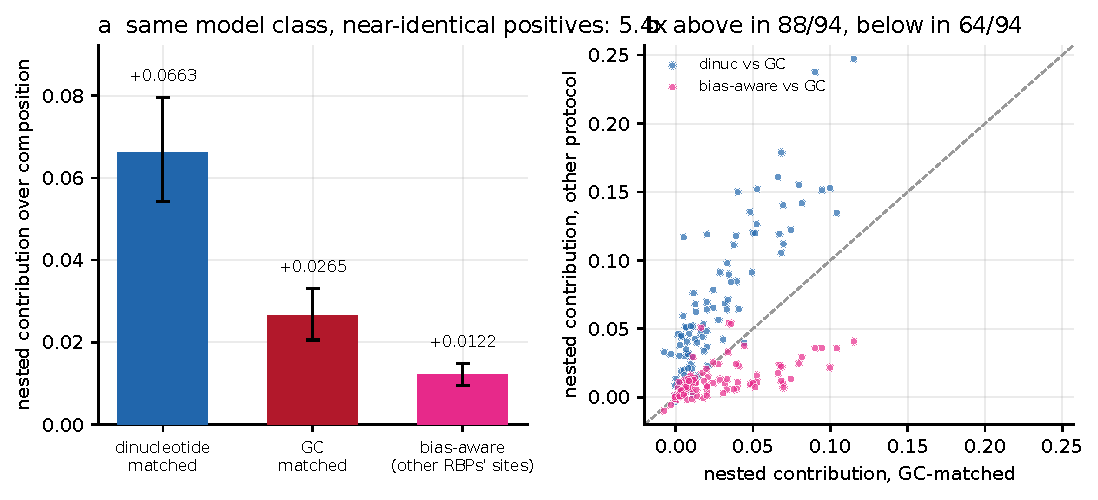
\includegraphics[width=\textwidth]{figures/f10_three_protocols}
\caption{\textbf{The three protocols, and the reversal.} Same 94 datasets, same positives, same 4-mer, same folds and same estimator; only the negatives differ. (a) Composition-only AUROC, apparent AUROC and nested contribution under each protocol. (b) Nested contribution per dataset, dinucleotide-matched against GC-matched, paired; points above the diagonal are the 88 of 94 datasets where the model contributes more under dinucleotide matching. (c) The same for the bias-aware arm against GC-matched, lower in 64 of 94. Apparent AUROC moves in the opposite direction to contribution: dinucleotide matching lowers it in 94 of 94 datasets.}
\label{fig:three}
\end{figure}

\subsection{No rescaling supplies a transportable protocol-free quantity}

AUROC is compressive near one, so a gain measured against a 0.82 baseline is arithmetically
smaller than the same gain against a 0.63 baseline, and part of the 5.42-fold span is scale
rather than protocol. We searched for a coordinate in which the span disappears
(Figure~\ref{fig:scale}).

Over eight monotone reparameterisations of the same 282 protocol-dataset cells, the span falls
but does not close. Somers' $D$ \citep{somers1962} is an affine map of AUROC and returns 5.42 by
construction, which serves as an internal control on the sweep. Every unbounded link reduces the
span, in the order of how aggressively it stretches the upper tail: arcsine 3.99, complementary
log-log 3.94, binormal $d'$ 3.18, logit 2.72. The smallest is obtained by dividing the
contribution by the baseline's own headroom, $1$ minus the composition AUROC, at 2.00
$[1.67, 2.46]$. Normalising instead by the excess over chance, which is the transformation a
reader is most likely to invent, makes the span far worse at 18.2, because the denominator itself
varies with protocol and approaches zero.

The 2.00 figure should not be compared against 1.0. A ratio of the largest to smallest of three
noisy means is bounded below by one and biased upward, so some span is expected under any
sampling. Simulating equal true arm means while preserving the real between-arm dataset pairing
gives a null with median 1.064 and 95th percentile 1.175. The observed 2.00 lies well outside
it, so the residual span is not an artefact of taking a ratio.

The headroom coordinate is not a coordinate, however, but a fitted member of a family, and we
report that rather than resting on it. Dividing by headroom is the $p=1$ case of dividing by
headroom raised to the power $p$, and our sweep stopped at exactly the member we recommend.
Extending the family, the span collapses:

\begin{table}[htbp]
\centering
\caption{Fold span across the three protocols for $g/(1-c)^{p}$, where $g$ is the nested
contribution and $c$ the composition AUROC. An equalising exponent exists in sample.}
\label{tab:exponent}
\begin{tabular}{lccccccc}
\toprule
$p$ & 0 & 0.5 & 1.0 & 1.25 & \textbf{1.544} & 1.75 & 2.0 \\
\midrule
span & 5.42 & 3.43 & 2.00 & 1.48 & \textbf{1.005} & 1.34 & 1.95 \\
\bottomrule
\end{tabular}
\end{table}

At $p=1.544$ the three protocols agree on the panel mean to within 0.5\%. A monotone rescaling
that equalises our three protocols therefore exists, and any claim that none does would be false
on our own data.

The exponent is a property of the benchmark rather than of the quantity, and that is the result.
Fitted to the two negative sets released by \citet{horlacher2023}, the equalising exponent is
3.649, a factor of 2.4 from ours. Our exponent leaves their benchmark at 2.340 against the 2.381
it started from, that is, it buys nothing there. So a normalisation strong enough to equalise one
benchmark must be refitted on the next, and the absence of a protocol-free measure is a
statement about transportability rather than about a floor. Stated that way it is testable, and
we have tested it on data we did not build.

\begin{figure}[htbp]
\centering
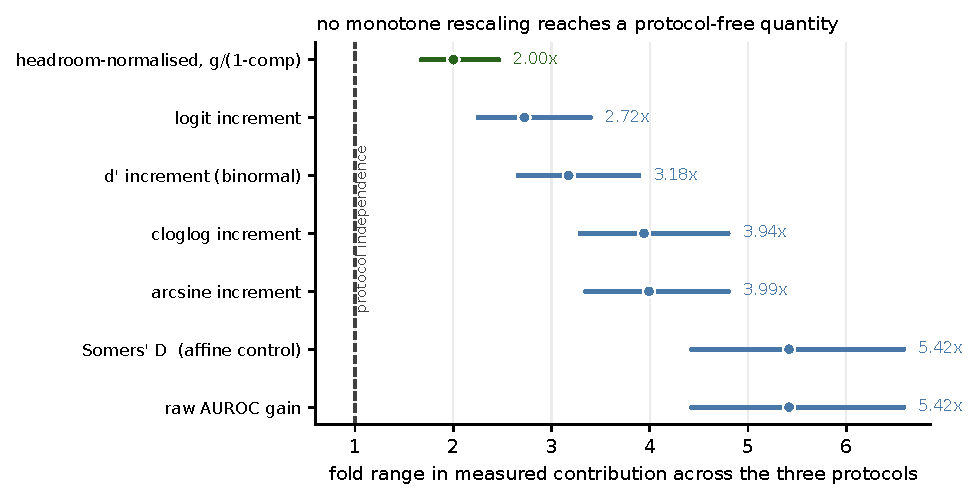
\includegraphics[width=0.72\textwidth]{figures/f11_scale_sweep}
\caption{\textbf{No rescaling reaches a protocol-free quantity among fixed coordinates.} Fold span in measured contribution across the three protocols under eight monotone reparameterisations of the same 282 protocol-dataset cells. Points are the span, bars are 95\% percentile intervals from a bootstrap over datasets (2000 draws), and the dashed line marks protocol independence. Somers' $D$ is an affine map of AUROC and returns the raw value by construction, serving as a control on the sweep. The minimum, 2.00 $[1.67,2.46]$, is attained by dividing by the baseline's own headroom.}
\label{fig:scale}
\end{figure}

\subsection{It is the composition baseline, not the protocol label}

Pooled across all 282 protocol-dataset cells the contribution tracks the composition baseline at
Spearman $-0.600$ ($p=6\times10^{-29}$). We report this as the mechanism rather than defending
against it: most of what a protocol does is decide how much room the baseline leaves. Three
analyses localise the effect (Figure~\ref{fig:baseline}).

\paragraph{Variance accounting.} Regressing the contribution on a cubic in the composition
baseline over all 282 cells and then adding protocol dummies, the protocol label adds 1.0\% of
variance given the baseline, while the baseline adds 11.0\% given the label: an order of
magnitude in the baseline's favour.

\paragraph{A natural experiment.} The bias-aware protocol usually raises the baseline relative
to GC matching, but in 27 of 94 datasets it lowers it. If the protocol label carried the
information, its deficit would persist there. It reverses: $-0.0212$ $[-0.0269, -0.0157]$ where
it raises the baseline, $+0.0028$ $[-0.0000, +0.0063]$ where it lowers it, with within-dataset
Spearman correlation between the change in baseline and the change in contribution of $-0.664$
($p=3\times10^{-13}$). Whichever protocol leaves the lower baseline yields the higher
contribution, regardless of which protocol it is.

\paragraph{Matching on the baseline.} Because the dinucleotide baseline is lower than the GC
baseline in 94 of 94 datasets, arm and baseline are perfectly rank-confounded within a dataset
and the comparison must borrow across datasets. Doing so, the headline $+0.0398$ falls to
$-0.0087$ $[-0.0265, +0.0122]$. We report this and also report why it is not a clean test: the 41
retained pairs are selected from opposing tails, the dinucleotide members having mean baseline
0.6875 against the panel's 0.6274 and the GC members 0.6904 against 0.7827; only 24 distinct GC
partners serve 41 comparisons, with one reused eleven times; and no protein matching is possible.
Nearest-neighbour matching on a variable monotonically related to the outcome, with reuse and
across proteins, is biased toward zero by construction here. The honest reading is that the
comparison is not identified for this pair, which is consistent with the pair's common support
being only 0.073 AUROC wide over 33 of 188 cells.

\paragraph{Where it is identified, a protocol-family residual survives.} The
GC-versus-bias-aware pair overlaps by 0.212 AUROC over 130 of 188 cells, so the same matched
design is straightforward there. Under two independent designs the bias-aware arm still costs
$-0.0081$ $[-0.0130, -0.0036]$ (nearest-baseline matching) and $-0.0043$ $[-0.0077, -0.0012]$
(within-dataset intercept at zero baseline shift). Decomposed by pair, the protocol label's
incremental variance is 0.05\% for GC versus dinucleotide but 3.40\% for GC versus bias-aware, so
the pooled 1.0\% averages a pair where the question is unanswerable with one where it is
answerable.

\paragraph{The mechanism, which changes the framing from three protocols to two families.} The
gradient from baseline to contribution is a property of composition-matched negatives and is
absent otherwise: within-arm Spearman is $-0.545$ (GC), $-0.462$ (dinucleotide) and $-0.122$,
not significant (bias-aware). Inside the composition-matched family the baseline is essentially
the whole story; across families it is not, and a residual of about 0.005 to 0.008 AUROC remains.
This is why we do not name headroom as the general mechanism.

\begin{figure}[htbp]
\centering
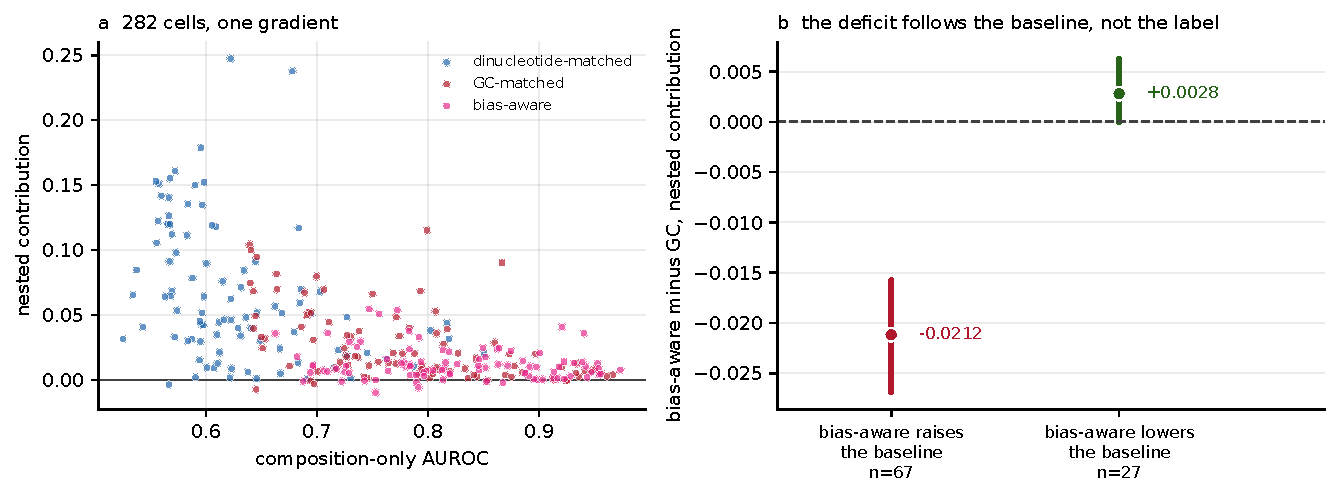
\includegraphics[width=\textwidth]{figures/f12_protocol_or_baseline}
\caption{\textbf{The composition baseline, not the protocol label.} (a) All 282 protocol-dataset cells: nested contribution against the composition-only AUROC the protocol left behind, coloured by protocol; pooled Spearman $-0.600$ ($p=6\times10^{-29}$). (b) The natural experiment. Datasets are split by whether the bias-aware protocol raised or lowered the composition baseline relative to GC matching ($n=67$ and $27$); points are stratum means and bars are 95\% percentile intervals from a bootstrap over datasets (4000 draws). The deficit reverses where the baseline falls.}
\label{fig:baseline}
\end{figure}

\subsection{The effect is not a property of the model class}

The GC arm was swept for two further architectures, 470 fold-runs each: a 7089-parameter
convolutional network in the style of \citet{alipanahi2015} and a fully fine-tuned
19.78~M-parameter SpliceBERT \citep{chen2024}, using the same folds, the same seed and the same
code path, with per-window scores committed (Figure~\ref{fig:models}).

\begin{table}[htbp]
\centering
\caption{The protocol contrast for three model classes, $n=94$ datasets, identical rows and
folds. Intervals are protein-clustered percentile intervals over the 79 proteins.}
\label{tab:models}
\begin{tabular}{lccc}
\toprule
model & GC arm & dinucleotide arm & contrast \\
\midrule
4-mer & $+0.0265$ & $+0.0663$ & $+0.0398$ $[+0.0325, +0.0477]$ \\
CNN & $+0.0330$ & $+0.0860$ & $+0.0530$ $[+0.0440, +0.0627]$ \\
SpliceBERT & $+0.0890$ & $+0.1754$ & $+0.0864$ $[+0.0778, +0.0951]$ \\
\bottomrule
\end{tabular}
\end{table}

The contrast is present for all three model classes on all 94 datasets, which retires the
objection that a five-fold span measured with a bag of $k$-mers is an artefact of a weak model:
it is still a factor of 2.4 for a fine-tuned transformer measured on the same rows.

We then swept both neural models on the bias-aware arm as well, so that the three-protocol
result and the multi-model result meet in the same cells rather than being two separate
two-way comparisons (Table~\ref{tab:threemodels}).

\begin{table}[htbp]
\centering
\caption{The full design: three negative-set protocols by three model classes, $n=94$ datasets,
identical rows and folds throughout. Spans are ratios of panel means with protein-clustered
percentile intervals.}
\label{tab:threemodels}
\begin{tabular}{lcccc}
\toprule
model & dinucleotide & GC & bias-aware & span \\
\midrule
4-mer & $+0.0663$ & $+0.0265$ & $+0.0122$ & 5.42 $[4.43, 6.58]$ \\
CNN & $+0.0860$ & $+0.0330$ & $+0.0113$ & \textbf{7.63} $[6.23, 9.63]$ \\
SpliceBERT & $+0.1754$ & $+0.0890$ & $+0.0466$ & 3.76 $[3.27, 4.34]$ \\
\midrule
composition alone & 0.6274 & 0.7827 & 0.8248 & \\
\bottomrule
\end{tabular}
\end{table}

Three things follow. The span is present for every model class, so it is a property of the
benchmark rather than of the model used to measure it, and the weakest of the three is still
3.76-fold. The bias-aware protocol yields the least for all three models while having the
highest composition baseline, so the reversal in the title is not specific to a $k$-mer. And
the span is \emph{widest for the convolutional network}, not for the largest model, which is the
same non-monotonicity in capacity that the ratio-scale multiplier shows: nothing here grows with
capacity. On the ratio
scale the ordering reverses, the multiplier being 3.08, 3.51 and 2.38 for the three models
(geometric mean over the 77 datasets positive in both arms for all models), so the contrast does
not grow with capacity and we make no such claim.

\paragraph{Whose property is the multiplier?} Decomposing its log over the 262 dataset-by-model
cells where both arms are positive, RBP identity accounts for 64.8\% of the variance, cell line
0.2\% and model class 2.8\%. Those shares are not directly comparable, because a factor with 79
levels absorbs 29.7\% of the variance of relabelled data while a three-level factor absorbs
0.8\%. Measured against a null that permutes protein labels between datasets while keeping each
dataset-by-model block intact, protein's excess is $+7.2$ points ($p=0.003$), and the direct test
is stronger than either share: the same protein's log multiplier agrees across the two cell lines
at $r=0.586$ (Spearman 0.594, $p=0.0001$) over 40 protein-by-model pairs. Cell line is not
detectable, though with only fifteen proteins in both lines the design has little power to
detect it. Model class is small but real ($p=0.023$), consistent with SpliceBERT's significantly
lower multiplier, and it survives the differential censoring visible in its own input.

\paragraph{Why we do not decompose the span into compression and a residual protocol effect.}
The natural next step is to transplant a model's discriminability increment across baselines and
call the unexplained part a protocol effect. That quantity is not identified for any of the three
models. Its central assumption, that the increment is invariant to the baseline it is measured
against, is violated in these data, and across a grid of twelve reasonable specifications only 4
of 6 sign tests hold for the 4-mer, 6 of 6 for the CNN and 1 of 6 for SpliceBERT. One standard
link, the log odds, reverses the sign entirely, which is the behaviour \citet{mood2010} describes
for odds ratios under unobserved heterogeneity. With three arms the transplant residual's sign
follows the direction of transport: carrying an increment from a high-baseline arm to a
low-baseline one gives $+0.0452$ and the reverse gives $-0.0259$. We therefore report the raw
contrast, which needs no transplant, no link and no transportability assumption, and treat the
decomposition as a sensitivity analysis whose failure is itself informative.

\paragraph{A provenance limitation on this section specifically.} For 20 of the 94 datasets in
the dinucleotide arm, the committed neural-network scores were produced under a partition that is
not chromosome-grouped: fold sizes were preserved, so no count-based check detects it, but up to
23 chromosomes appear in a single fold and up to 44.5\% of rows have a same-strand neighbour
within 1~kb assigned to a different fold, against exactly zero under the study folds and zero
throughout the GC arm. The 4-mer is refit on the study folds for every dataset and so is
unaffected, which makes it a clean internal control. Restricting the neural comparison to the 74
correctly partitioned datasets gives contrasts of $+0.0436$ (4-mer), $+0.0506$ (CNN) and
$+0.0878$ (SpliceBERT), all within the protein-clustered interval half-widths of
Table~\ref{tab:models}. We report the 74-dataset figures as primary for the two neural models and
the 94-dataset figures as a sensitivity.

A second asymmetry in the same section, disclosed for completeness: the 4-mer entered the nested
fit as a log odds and the neural models as probabilities, and a logistic regression is not
invariant to a nonlinear transform of a covariate. Refitting the neural arms on the logit scale
raises their contributions by $+0.0008$ (CNN) and $+0.0030$ (SpliceBERT) on the GC arm, so the
published values are conservative, and moves the contrasts by at most 0.0004. AUROC is invariant
to monotone transforms, so no standalone AUROC is affected.

\begin{figure}[htbp]
\centering
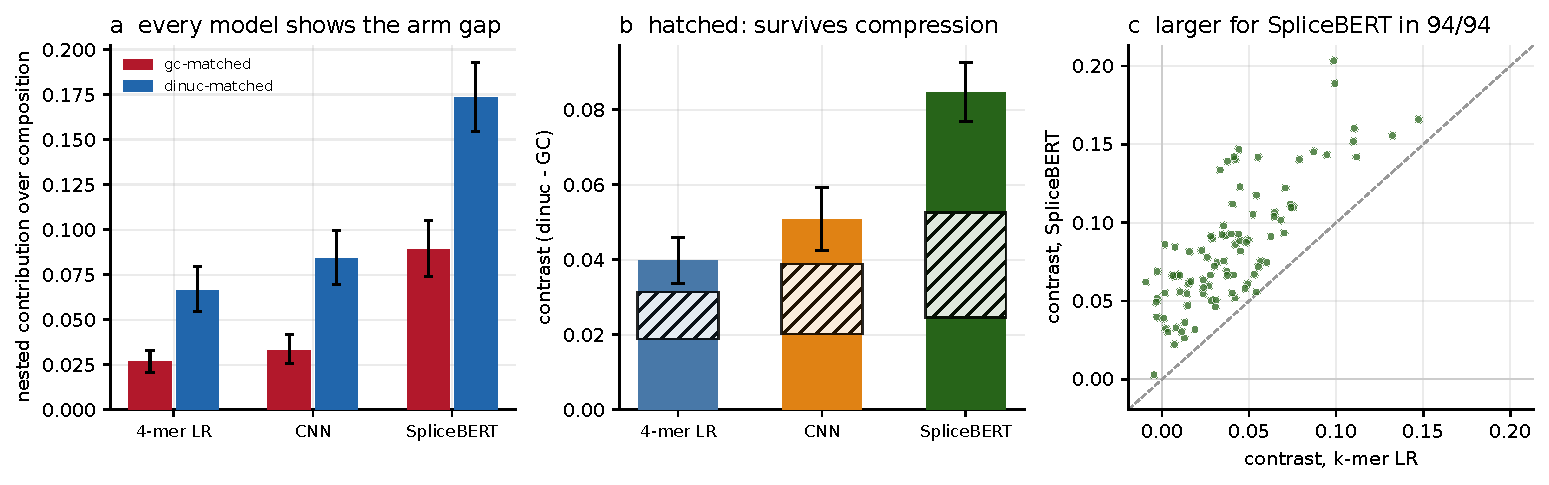
\includegraphics[width=\textwidth]{figures/f9_deep_contrast}
\caption{\textbf{The contrast holds for three model classes.} Nested contribution in each arm for a 4-mer logistic regression, a 7089-parameter convolutional network and a fully fine-tuned 19.78~M-parameter SpliceBERT, on identical rows and folds, $n=94$. Intervals are 95\% percentile intervals from a bootstrap over the 79 proteins, taking all datasets of each sampled protein (4000 draws). On the ratio scale the ordering reverses, so the contrast does not grow with capacity.}
\label{fig:models}
\end{figure}

\subsection{The calibration replicates on an independent benchmark}

Every result above is measured on windows we built. To test whether any of it travels we applied
the identical decomposition to the negative sets released by \citet{horlacher2023}: their
positives, their peak calling, their negative-set construction and their fold assignments, over
the 45 datasets shared with our panel. Only the measurement is ours
(Figure~\ref{fig:external}).

\begin{table}[htbp]
\centering
\caption{The same decomposition on an independent benchmark, $n=45$ datasets. Their positives,
negatives and folds.}
\label{tab:external}
\begin{tabular}{lccc}
\toprule
their negative set & composition & apparent & contribution \\
\midrule
negative-1 (transcript background) & 0.8211 & 0.8606 & $+0.0395$ \\
negative-2 (other RBPs' sites) & 0.7560 & 0.7726 & $+0.0166$ \\
\bottomrule
\end{tabular}
\end{table}

The span on their benchmark is 2.381, against 2.17 for the family-matched pair in our own data,
the GC versus bias-aware comparison; their negative-2 is constructed like our bias-aware arm, so
that is the correct comparison rather than our dinucleotide-versus-GC 2.50.

More importantly, the two-family mechanism replicates arm for arm. The within-arm gradient from
baseline to contribution on their data is $-0.645$ ($p=1.8\times10^{-6}$) for their
composition-matched transcript-background arm and $-0.187$ ($p=0.22$, not significant) for their
other-RBPs'-sites arm, against $-0.545$ and $-0.462$ for our composition-matched arms and
$-0.122$, not significant, for ours. An independent laboratory's negatives and folds reproduce
both the presence of the gradient in one family and its absence in the other.

This also explains the one feature of their benchmark that is anti-monotone to ours: their
negative-2 has both the lower baseline and the lower contribution, which no single-family
headroom relation predicts and which a cross-family residual does.

\begin{figure}[htbp]
\centering
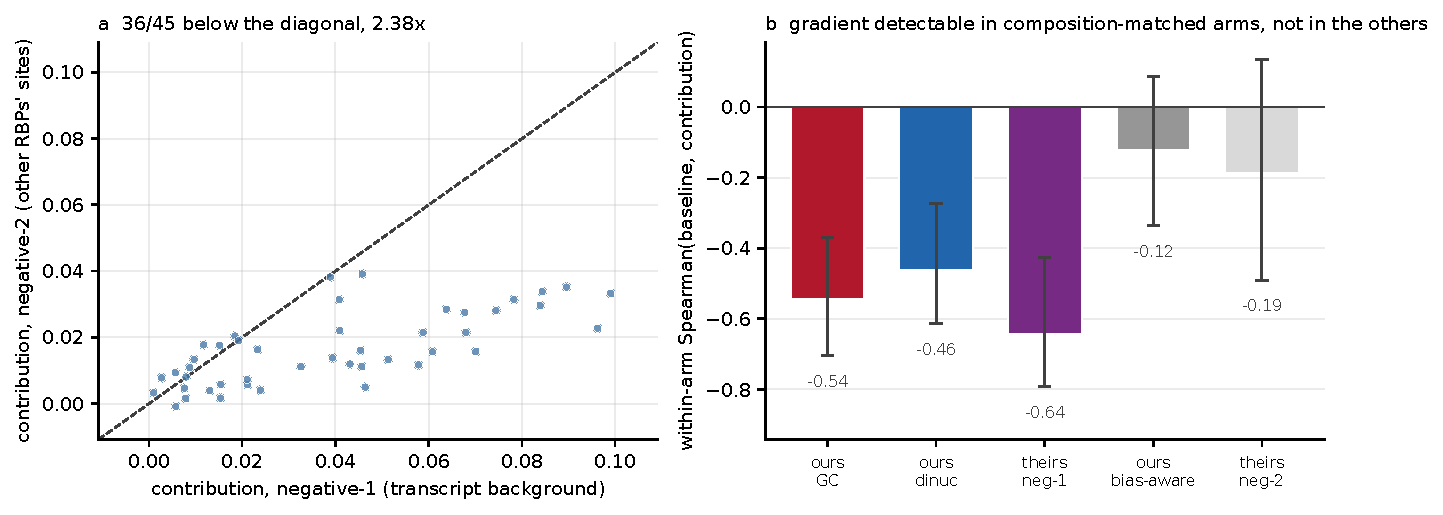
\includegraphics[width=\textwidth]{figures/f14_external_validation}
\caption{\textbf{Replication on an independent benchmark.} \citet{horlacher2023}'s released negative sets, their peak calling and their folds, over the 45 datasets shared with our panel; only the measurement is ours. (a) Nested contribution under their negative-2 against their negative-1, paired per dataset; 36 of 45 fall below the diagonal. (b) The mechanism, which is what travels: the within-arm gradient from composition baseline to contribution, for the composition-matched arms in both benchmarks and the other-RBPs'-sites arms in both. The gradient is present in one family and absent in the other, in both benchmarks independently.}
\label{fig:external}
\end{figure}

\subsection{The recommendation, and the limits of what it buys}

The deliverable is a two-number report: state the composition-only AUROC obtained under the same
protocol beside every headline AUROC. Everything above shows that not doing so is a problem.
Whether doing so helps is a separate question, and we tested it by putting a reader in the
position the recommendation is meant to rescue, holding two papers that used different protocols
and wanting to compare what the models contributed (Figure~\ref{fig:recommendation}).

On our data, normalising by headroom improves rank agreement in 3 of 3 protocol pairs and reduces
disagreement on a common scale in 3 of 3, by 58\%, 10\% and 48\%. Rank agreement is scale-free,
so no normalisation can flatter it.

Two findings qualify this. First, only the GC-versus-dinucleotide rank improvement has an
interval clear of zero ($+0.051$ $[+0.007, +0.115]$); the other two pairs are consistent in
direction and individually null. That pair is precisely the one where the protocol label adds
0.05\% of variance, so the fix is best demonstrated where it is least needed. Second, and
decisively, the test fails to replicate out of sample. On the 45 datasets of
\citet{horlacher2023}, rank agreement \emph{falls} from 0.706 to 0.656 under normalisation and
disagreement \emph{rises} from 0.860 to 0.908. Those are, verbatim, the two criteria we
pre-registered as falsifying. The change in rank agreement is $-0.050$ $[-0.222, +0.140]$, so at
$n=45$ this is a failure to replicate rather than a refutation, but it points the wrong way and
we report it.

We therefore make the weaker claim that the evidence supports. Report the composition-only AUROC
under the same protocol, because it is the only summary of what the protocol did that a reader
can act on and because it makes the problem visible. Do not treat any normalisation as making
contributions comparable across protocols: we cannot demonstrate that it does, and on
independent data it does not. The operational recommendation is to report the baseline and to
refrain from cross-protocol comparison, not to rescale and proceed.

\begin{figure}[htbp]
\centering
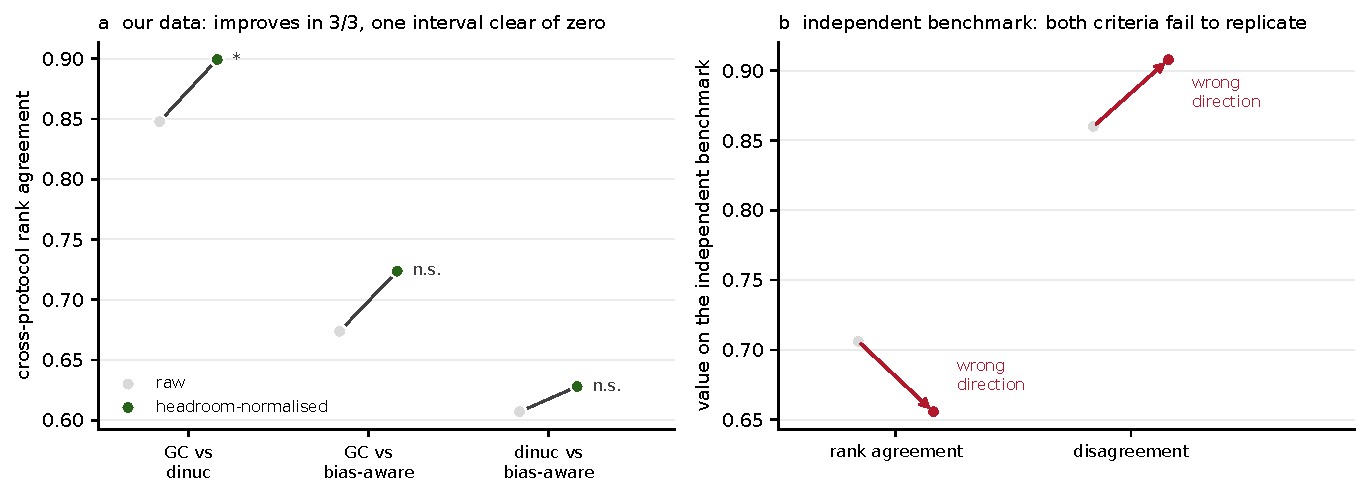
\includegraphics[width=\textwidth]{figures/f15_recommendation}
\caption{\textbf{The recommendation, and where it stops working.} (a) On our data, cross-protocol rank agreement before and after dividing by the baseline's headroom, for each protocol pair. Agreement improves in 3 of 3, but only the GC-versus-dinucleotide improvement has a protein-clustered interval clear of zero. (b) The same test on the independent benchmark of Figure~\ref{fig:external}, $n=45$: rank agreement falls and disagreement rises under normalisation, which are the two criteria pre-registered as falsifying the recommendation. The change in rank agreement is $-0.050$ $[-0.222,+0.140]$, so this is a failure to replicate rather than a refutation.}
\label{fig:recommendation}
\end{figure}


\section{Discussion}
This study shows that a sequence model's incremental performance is not determined by the model
alone. When the same source peaks were used and the model class, fold assignment and estimator were held fixed, changing
the construction of the negative set altered the estimated contribution of a 4-mer model by
5.42-fold under the conventional two-stage estimator and by 4.84-fold under the primary
cross-fitted estimator. The corresponding two-stage spans ranged from 3.7- to 7.4-fold across
three model classes. Within the study panel, the protocol yielding the lowest apparent AUROC produced
the largest increment over composition, whereas the protocol yielding the highest apparent
AUROC produced the smallest increment. Negative-set construction therefore changes both the
difficulty of the task and the quantity being measured; the two should not be treated as
interchangeable indicators of stringency.

Five reporting practices follow from these results.

\begin{enumerate}\setlength{\itemsep}{2pt}
\item \textbf{Describe how negatives were constructed.} The candidate pool, matching variables,
  tolerances, achieved match quality and unconstrained covariates should be reported in enough
  detail to reproduce the set. Nominal tolerances alone did not capture the achieved matching
  in the study data.
\item \textbf{Report the composition-only AUROC under the same protocol.} This baseline is
  inexpensive to fit and provides a direct measure of the discrimination available from
  composition. In the bias-aware arm, the 19-feature composition model outperformed the 4-mer
  in 53 of 94 datasets.
\item \textbf{State the order of the composition baseline.} Incremental performance is defined
  relative to the features already represented. Raising the baseline from dinucleotide to
  trinucleotide composition reduced every contribution, although protocol dependence remained.
\item \textbf{Confirm that the baseline remains estimable as its order increases.} In this panel,
  out-of-fold baseline performance improved through order three but not at order four. Beyond that
  point, apparent increments can reflect estimation error in the baseline rather than additional
  information in the sequence model.
\item \textbf{Calibrate the estimator with a null model.} A 2-mer model provides such a control
  because its information is already contained in the dinucleotide baseline. The conventional
  estimator nevertheless returned $+0.0111$ to $+0.0137$ (Section~\ref{sec:floor}), showing that
  increments of this magnitude cannot be interpreted without an estimator-specific null.
\end{enumerate}

These recommendations imply that contributions estimated under different negative-set
protocols should not be compared directly. Each protocol defines a different classification
problem, and an increment is meaningful only relative to the baseline and observations used to
estimate it.

The bias-aware protocol illustrates why this distinction matters. Drawing negatives from sites
bound by other RBPs can reduce broad accessibility and composition artefacts, but it also poses
a biologically different task from separating bound sites from genomic background. RBPs differ
in their preferred transcript regions, and transcript regions have characteristic nucleotide
composition. Stratifying the donor draw by region reduced the bias-aware composition baseline
by 0.020 AUROC, accounting for 46\% of its excess over the GC arm, and decreased its measured
contribution by approximately one quarter. The arm nevertheless remained the lowest of the
three in incremental performance. Thus, transcript region explains part, but not all, of the
bias-aware baseline. This is not an argument against bias-aware negatives; it shows that their
results answer a different question and require protocol-specific interpretation.

No standard reparameterisation made the contributions comparable across protocols. Dividing by
the baseline's remaining headroom reduced the span, but the fitted exponent depended on the
aggregation rule, benchmark and model class. It therefore cannot serve as a transferable
normalisation. The protocol ordering was also preserved for likelihood-ratio statistics,
McFadden's $R^2$, average precision and integrated discrimination improvement. The magnitude
was scale-dependent: for the 4-mer, the three-protocol span was 5.42-fold in AUROC and
approximately two-fold on the unbounded scales. The qualitative dependence is consequently not
an artefact of the AUROC ceiling, although the headline fold change is specific to the AUROC
scale.

The baseline order introduces a second source of dependence. A 4-mer model evaluated against a
trinucleotide baseline largely measures the remaining fourth-order composition rather than a
general notion of motif recognition. Increasing the baseline order is therefore informative but
not neutral: it is structurally less favourable to $k$-mer models than to models that can use
position or longer-range context. I interpret these analyses as a characterisation of what the
baseline absorbs, not as a model-capacity ranking.

These findings extend the observation by \citet{horlacher2023} that negative-set construction
changes apparent RBP-prediction performance. The present analysis shows that the same choice also
changes incremental performance relative to an explicit baseline. In the study panel, the magnitude
of protocol-associated variation was comparable to that produced by changing model class:
within-protocol model spans were 2.62- to 4.14-fold, whereas within-model protocol spans were
3.7- to 7.4-fold. Similar sensitivity has been reported in transcription-factor binding
prediction \citep{tourne2026}, suggesting that the issue may extend beyond eCLIP, although the
current study does not test that generalisation directly.

\subsection*{Limitations}

The estimated magnitudes are conditional on the 19-feature mono- and dinucleotide baseline.
Every contribution decreased when the baseline was extended to trinucleotides, while the
protocol ordering persisted. The existence of protocol dependence was therefore robust to the
tested baseline orders, but its size was not. Neither the present data nor a transformation can
define a protocol-independent contribution.

The conventional two-stage estimator introduced an additional limitation. For a 2-mer model
whose information is contained in the baseline, it produced a positive contribution rather than
the expected zero. The source was an information route between the inner score generation and
outer evaluation folds. Cross-fitting the score covariate reduced the floor by at least 95\%
in every arm and narrowed the 4-mer span from 5.42-fold to 4.84-fold without removing it. This
correction was not run for the convolutional network or SpliceBERT because it would require new
neural training. Their spans are therefore exploratory two-stage estimates and should not be
compared numerically with the primary cross-fitted 4-mer result.

External validation supports the general dependence on negative-set construction but narrows
its interpretation. In 135 datasets from \citet{horlacher2023} that were absent from the study panel,
the two negative sets produced a 1.69-fold two-stage span (95\% CI 1.41--2.03) and a 1.66-fold
cross-fitted span (1.40--1.98). Chromosome-blocked refolding gave corresponding estimates of
1.73 (1.43--2.10) and 1.67 (1.40--2.00). These datasets did not overlap the study datasets, but 31 of the
108 proteins overlapped;
excluding all shared proteins still gave a 1.66-fold span. The analysis is therefore external in
dataset construction and processing, not in assay, organism or all biological entities. It
remains ENCODE eCLIP from K562 and HepG2 cells.

The inverse relation between apparent difficulty and incremental contribution did not replicate
externally. In the Horlacher benchmark, the more difficult arm also yielded the smaller
contribution, and the per-dataset association was null. The transferable result is therefore
that negative-set construction changes the measured contribution, not that apparent AUROC and
contribution must move in opposite directions. The external benchmark was also known before the
held-out subset was scored. Its criteria were specified before analysis of that subset, but the
study should not be interpreted as a prospective search across independent benchmarks.

The study covers three model classes, two cell lines and one assay. The 4-mer model, small
convolutional network and 19.78~M-parameter SpliceBERT form a capacity ladder rather than a
survey of published RBP predictors. No model larger than 20~M parameters was tested. The
cross-protocol training and evaluation analysis (Section~\ref{sec:transport}) was limited to the
4-mer; extending it to the neural models would require retraining. Its off-diagonal cells also combine a protocol change
with distribution shift, so the estimated training and evaluation shares are descriptive and
not causal.

Several design choices were fixed before analysis. All primary arms used a 1:1 class ratio,
whereas genome-wide applications are much more imbalanced. AUROC is prevalence-invariant, but
precision-based measures are not. Sensitivity analyses at 1:2, 1:4 and 2:1 preserved the
protocol ordering, although the magnitudes varied. Window length was fixed at 101~nt and was not
systematically varied. A longer window would provide more sequence for estimating composition
and could alter both baseline and incremental performance.

Chromosome-blocked folds prevent loci from being divided across training and test sets, but they
do not eliminate similarity between homologous loci on different chromosomes. Only 176 of
2.7 million windows belonged to gene names represented in more than one fold, primarily
pseudo-autosomal and multicopy small-RNA genes. Gene-clustered refitting changed the two-arm
contrast by $0.0003$. Three alternative chromosome assignments varied it by $0.00058$. These
results indicate limited sensitivity to the fold assignment for the 4-mer, but the neural models
were evaluated only on the frozen chromosome partition.

Window centring had a larger effect. The discriminative signal occurred a median of 23~nt from
the peak midpoint, and summit-centred windows could not be tested because the required summit
field was absent from the examined peak files. Across midpoint, transcript-oriented boundary
and displaced-midpoint definitions, the two-arm contrast varied by $0.0077$ in ten datasets.
The published midpoint definition produced the largest of the three estimates, so window
centring remains an important source of uncertainty.

Negative construction is stochastic. Independent redraws changed panel means less than the
between-protein sampling uncertainty: incorporating draw variability increased interval widths
by 0.49--0.81\% in the composition-matched arms and by 3.6\% in the bias-aware arm. The
ordering of protocols was unchanged. For the composition-matched arms, redraws condition on the
positive windows retained by the original matching pass and therefore quantify variability in
negative selection rather than the complete construction process.

Neural-model initialisation was not seeded across the 2830 committed fold runs. A repeated CNN
fit on one dataset, using identical observations and folds on two hardware platforms, produced
per-window score correlations of 0.9903 and fold-AUROC differences no larger than 0.0007. This
experiment combines hardware and initialisation effects and does not establish complete neural
reproducibility. All downstream analyses are deterministic given the released scores.

The positive sets in the two composition-matched arms were nearly, but not perfectly,
identical because a positive was discarded when its matcher found no acceptable negative. Their
median Jaccard similarity was 0.9972. Restricting both arms to the common positive set removed
0.23\% of positives and changed the contrast from $+0.0398$ to $+0.0401$, preserving its sign
in the same 88 of 94 datasets. Because matching failures are composition-dependent, this
intersection analysis is a sensitivity check rather than the primary estimand.

Finally, the released ENCODE peaks were already thresholded, and I applied no additional
significance filter. Fixed 101-nt windows discard peak width and may omit the crosslink site for
wide peaks. Negatives were not filtered by gene expression, and transcript region was assigned
from the window midpoint under a fixed annotation precedence. These choices may affect the
absolute measurements even though the same rules were applied across the paired protocols where
applicable.

The repository's verification suite provides regression and provenance checks, not independent
confirmation of the original analysis. Most assertions compare reported values with committed
evidence from the same run; two checks independently reconstruct 285 AUROCs from per-window
scores and the headline contrast from raw sequence. The manuscript-number trace can identify an
unsupported value but cannot determine whether a valid value has been attached to the correct
claim. These safeguards reduce transcription and drift errors, but scientific validity still
depends on the design, assumptions and limitations described above.


\section{Conclusion}
The contribution of an RBP sequence model beyond nucleotide composition depends jointly on the
model, the baseline and the negative-set protocol. In the study panel, the protocol yielding the
highest apparent AUROC left the least incremental signal for the sequence model, while stricter
composition matching lowered apparent AUROC and increased the measured contribution. The
protocol-associated variation was comparable in scale to that produced by changing model
class.

Estimator design also mattered. The conventional two-stage procedure returned a positive
increment for a model whose information was already contained in the baseline. Cross-fitting
the score covariate reduced this null floor by at least 95\% and preserved a 4.84-fold span
across protocols. The externally constructed benchmark reproduced the protocol dependence, but
not the inverse relation between apparent difficulty and contribution.

These findings support a practical reporting standard. Studies should describe the negative-set
construction in reproducible detail, report the composition-only performance under the same
protocol, state the baseline order, and calibrate the incremental estimator with a null model.
Score covariates should be cross-fitted when feasible. Most importantly, contributions measured
under different negative-set protocols should not be interpreted as directly comparable. The
negative set is part of the scientific question posed by the benchmark, not merely a technical
setting used to evaluate it.


\backsection{Data availability}
All primary data are public. Positive windows derive from ENCODE eCLIP narrowPeak files
\citep{encode2012,vannostrand2020}; every dataset used, with its ENCFF file accession and ENCSR
experiment accession, is listed in Supplementary Table S1 (95 datasets, 79 proteins, 95
experiments). Gene annotation is GENCODE v45 \citep{frankish2023}. Cell-line expression used in
the transcription control comes from four ENCODE polyA RNA-seq quantification files:
ENCFF286KKZ and ENCFF829LCN for K562 (ENCSR115PIZ), and ENCFF863QWG and ENCFF376IXQ for HepG2
(ENCSR245ATJ and ENCSR813BDU). The external validation uses the negative sets and fold
assignments released by \citet{horlacher2023} at \doi{10.5281/zenodo.10600977}, downloaded and
md5-verified.

\texttt{results/tables/raw\_inputs.csv} records all 251 staged objects, including file size,
base64 MD5, storage timestamp, source URL, assembly and annotation release. The recorded sizes
and checksums match the stored objects, and the 244 peak files cover every accession in
Supplementary Table S1. The timestamps refer to writes to the project storage bucket, not to
provider download times. Because provider checksums were not recorded during retrieval, the MD5
values identify the files used in this study but do not independently verify the bytes served by
ENCODE or GENCODE. URL provenance is recorded explicitly for each object.

Derived data are released with the code under CC BY 4.0, including per-window out-of-fold scores
for all three model classes and all per-dataset result tables. Intermediate window tables that
contain genomic sequence are not redistributed. Given a reference genome and cloud credentials,
\texttt{./run.sh all} rebuilds the dinucleotide arm from the listed accessions. The GC and
bias-aware neural sweeps use separate drivers under \texttt{cloud/modal/}; their per-window
scores are included in the release. \texttt{results/tables/PROVENANCE.csv} classifies each table
by whether it is reproducible from raw inputs, recomputable from released evidence, a frozen
input, or dependent on the window store.

Supplementary Table S1 lists all 95 panel datasets. One of them, NCBP2 in K562, did not clear
the out-of-fold pair floor in the GC arm, so it carries no three-protocol results; its
\texttt{in\_three\_arm\_panel} field is false and its result columns are empty.

% BOTH DOIs, deliberately. The VERSION DOI identifies the exact snapshot the reported numbers
% came from, which is what a reproducibility citation needs. The concept DOI resolves to
% whichever version is latest, so it aids discovery and cannot identify this research object.
A permanently archived snapshot of the code and derived data is deposited at Zenodo. This
version, tag v1.0.0, is \doi{10.5281/zenodo.22679285}, and all versions resolve through
\doi{10.5281/zenodo.22679284}. That deposit is the tagged release of the repository named
below, so the archived snapshot and the state that produced these numbers are the same
object.


\backsection{Code availability}
The exact snapshot these results come from is archived at \doi{10.5281/zenodo.22679285}
(tag v1.0.0; all versions: \doi{10.5281/zenodo.22679284}).
All analysis code is available in the
\href{https://github.com/NirmalKumar31/rbp-protocol-calibration}{project repository} under the MIT licence, with
\texttt{results/} and \texttt{data/evidence/} under CC BY 4.0. The repository includes a
documented analysis environment, automated checks of reported values, and end-to-end
recomputations of 285 AUROCs from per-window scores and of the headline contrast from raw
sequence. \texttt{results/tables/PROVENANCE.csv} identifies the evidence available for each
released table. Reproducing the block-bootstrap design effect additionally requires genomic
coordinates from the regenerated window store.

\backsection{Use of AI tools}
I used generative AI tools (Anthropic Claude and OpenAI Codex) for coding and editorial
assistance. I reviewed their outputs and take full responsibility for this work.

\backsection{Acknowledgements}
I thank Horlacher and colleagues for making their processed negative sets and fold assignments
publicly available, which enabled the external validation in this study.

\backsection{Funding}
This research received no external funding.

\backsection{Competing interests}
I declare no competing interests.

\backsection{Ethics}
This study is a secondary analysis of publicly released data. It involved no human participants,
no animals and no identifiable personal information, so no ethical approval was required. The
ENCODE eCLIP experiments and the GENCODE annotation were produced and released by their
respective consortia under their own governance; this work reanalyses those public releases and
generated no new experimental data.

\begin{thebibliography}{20}

\bibitem[ENCODE Project Consortium(2012)]{encode2012}
ENCODE Project Consortium.
\newblock An integrated encyclopedia of DNA elements in the human genome.
\newblock \emph{Nature}, 489:57--74, 2012.
\newblock \doi{10.1038/nature11247}

\bibitem[Van Nostrand et~al.(2016)]{vannostrand2016}
E.~L. Van Nostrand, G.~A. Pratt, A.~A. Shishkin, et~al.
\newblock Robust transcriptome-wide discovery of RNA-binding protein binding sites with enhanced
CLIP (eCLIP).
\newblock \emph{Nature Methods}, 13:508--514, 2016.
\newblock \doi{10.1038/nmeth.3810}

\bibitem[Van Nostrand et~al.(2020)]{vannostrand2020}
E.~L. Van Nostrand, P.~Freese, G.~A. Pratt, et~al.
\newblock A large-scale binding and functional map of human RNA-binding proteins.
\newblock \emph{Nature}, 583:711--719, 2020.
\newblock \doi{10.1038/s41586-020-2077-3}

\bibitem[Horlacher et~al.(2023)]{horlacher2023}
M.~Horlacher et~al.
\newblock A systematic benchmark of machine learning methods for protein-RNA interaction
prediction.
\newblock \emph{Briefings in Bioinformatics}, 24(5):bbad307, 2023.
\newblock \doi{10.1093/bib/bbad307}

\bibitem[Frankish et~al.(2023)]{frankish2023}
A.~Frankish, S.~Carbonell-Sala, M.~Diekhans, et~al.
\newblock GENCODE: reference annotation for the human and mouse genomes in 2023.
\newblock \emph{Nucleic Acids Research}, 51(D1):D942--D949, 2023.
\newblock \doi{10.1093/nar/gkac1071}

\bibitem[Grimm et~al.(2015)]{grimm2015}
D.~G. Grimm, C.~A. Azencott, F.~Aicheler, et~al.
\newblock The evaluation of tools used to predict the impact of missense variants is hindered by
two types of circularity.
\newblock \emph{Human Mutation}, 36(5):513--523, 2015.
\newblock \doi{10.1002/humu.22768}

\bibitem[Whalen et~al.(2022)]{whalen2022}
S.~Whalen, J.~Schreiber, W.~S. Noble, and K.~S. Pollard.
\newblock Navigating the pitfalls of applying machine learning in genomics.
\newblock \emph{Nature Reviews Genetics}, 23:169--181, 2022.
\newblock \doi{10.1038/s41576-021-00434-9}

\bibitem[DeLong et~al.(1988)]{delong1988}
E.~R. DeLong, D.~M. DeLong, and D.~L. Clarke-Pearson.
\newblock Comparing the areas under two or more correlated receiver operating characteristic
curves: a nonparametric approach.
\newblock \emph{Biometrics}, 44:837--845, 1988.
\newblock \doi{10.2307/2531595}

\bibitem[Sun and Xu(2014)]{sun2014}
X.~Sun and W.~Xu.
\newblock Fast implementation of DeLong's algorithm for comparing the areas under correlated
receiver operating characteristic curves.
\newblock \emph{IEEE Signal Processing Letters}, 21(11):1389--1393, 2014.
\newblock \doi{10.1109/LSP.2014.2337313}

\bibitem[Somers(1962)]{somers1962}
R.~H. Somers.
\newblock A new asymmetric measure of association for ordinal variables.
\newblock \emph{American Sociological Review}, 27(6):799--811, 1962.
\newblock \doi{10.2307/2090408}

\bibitem[Firth(1993)]{firth1993}
D.~Firth.
\newblock Bias reduction of maximum likelihood estimates.
\newblock \emph{Biometrika}, 80(1):27--38, 1993.
\newblock \doi{10.1093/biomet/80.1.27}

\bibitem[Mood(2010)]{mood2010}
C.~Mood.
\newblock Logistic regression: why we cannot do what we think we can do, and what we can do about
it.
\newblock \emph{European Sociological Review}, 26(1):67--82, 2010.
\newblock \doi{10.1093/esr/jcp006}

\bibitem[Alipanahi et~al.(2015)]{alipanahi2015}
B.~Alipanahi, A.~Delong, M.~T. Weirauch, and B.~J. Frey.
\newblock Predicting the sequence specificities of DNA- and RNA-binding proteins by deep
learning.
\newblock \emph{Nature Biotechnology}, 33:831--838, 2015.
\newblock \doi{10.1038/nbt.3300}

\bibitem[Maticzka et~al.(2014)]{maticzka2014}
D.~Maticzka, S.~J. Lange, F.~Costa, and R.~Backofen.
\newblock GraphProt: modeling binding preferences of RNA-binding proteins.
\newblock \emph{Genome Biology}, 15:R17, 2014.
\newblock \doi{10.1186/gb-2014-15-1-r17}

\bibitem[Chen et~al.(2024)]{chen2024}
K.~Chen, Y.~Zhou, M.~Ding, et~al.
\newblock Self-supervised learning on millions of primary RNA sequences from 72 vertebrates
improves sequence-based RNA splicing prediction.
\newblock \emph{Briefings in Bioinformatics}, 25(3):bbae163, 2024.
\newblock \doi{10.1093/bib/bbae163}

\bibitem[Harris et~al.(2020)]{numpy}
C.~R. Harris, K.~J. Millman, S.~J. van~der Walt, et~al.
\newblock Array programming with NumPy.
\newblock \emph{Nature}, 585:357--362, 2020.
\newblock \doi{10.1038/s41586-020-2649-2}

\bibitem[Virtanen et~al.(2020)]{scipy}
P.~Virtanen, R.~Gommers, T.~E. Oliphant, et~al.
\newblock SciPy 1.0: fundamental algorithms for scientific computing in Python.
\newblock \emph{Nature Methods}, 17:261--272, 2020.
\newblock \doi{10.1038/s41592-019-0686-2}

\bibitem[Pedregosa et~al.(2011)]{sklearn}
F.~Pedregosa, G.~Varoquaux, A.~Gramfort, et~al.
\newblock Scikit-learn: machine learning in Python.
\newblock \emph{Journal of Machine Learning Research}, 12:2825--2830, 2011.

\bibitem[Paszke et~al.(2019)]{pytorch}
A.~Paszke, S.~Gross, F.~Massa, et~al.
\newblock PyTorch: an imperative style, high-performance deep learning library.
\newblock In \emph{Advances in Neural Information Processing Systems 32}, pages 8024--8035, 2019.

\bibitem[Hunter(2007)]{matplotlib}
J.~D. Hunter.
\newblock Matplotlib: a 2D graphics environment.
\newblock \emph{Computing in Science and Engineering}, 9(3):90--95, 2007.
\newblock \doi{10.1109/MCSE.2007.55}

\end{thebibliography}


\end{document}
